\documentclass[aspectratio=169]{beamer}
\setbeamertemplate{navigation symbols}{}
\usepackage{color,amsmath,comment, subfigure}
\usepackage{booktabs}
\usepackage{url}

\def\imagetop#1{\vtop{\null\hbox{#1}}} %http://tex.stackexchange.com/questions/23521/tabular-vertical-alignment-to-top

%\setbeameroption{show notes}

%%%%%%%%%%%%%%%%%%%%%%%%%%
\title[]{Class 16: Experimental studies of contagion}
\author[]{Matthew J. Salganik}
\institute{Sociology 204: Social Networks\\Princeton University}
\date[]{
1/3 Background
\vfill

\begin{flushleft}
\vspace{0.6in}

\includegraphics[width=0.1\textwidth]{figures/cc.png}
\end{flushleft}
}

%%%%%%%%%%%%%%%%%%%%%%%%%%%
% SWBAT Describe the challenge of isolating contagion from other causes of similarity
% SWBAT Describe different designs to measure social contagion
% SWBAT Use ideas of internal validity and external validity to identify concerns with experiments
% SWBAT TODO
%%%%%%%%%%%%%%%%%%%%%%%%%%%%%%%%%%%%%%%%%%
\begin{document}
\frame{\titlepage}
%%%%%%%%%%%%%%%%%%%%%%%%%%%
\begin{frame}

\begin{itemize}
\item ``birds of a feather flock together'' but why? \pause
\item Experiments are powerful ways to isolate and estimate causal effects \pause
\item Experiments are powerful but not perfect: internal validity, external validity, and ethics 
\end{itemize}

\end{frame}
%%%%%%%%%%%%%%
\begin{frame}

People are often similar to the people they are connected to socially\pause
\begin{itemize}
\item selection (like people become friends) \pause
\item shared environment \pause
\item contagion
\end{itemize}
\vfill
\pause
For some traits, selection dominates (e.g., gender). \pause For other traits, all might be at work.
\end{frame}
%%%%%%%%%%%%%%%%%%%%
\begin{frame}

\begin{itemize}
\item ``birds of a feather flock together'' but why? 
\item \textcolor{blue}{Experiments are powerful ways to isolate and estimate causal effects}
\item Experiments are powerful but not perfect: internal validity, external validity, and ethics 
\end{itemize}

\end{frame}
%%%%%%%%%%%%%%
\begin{frame}

``It's like you don't harass women, you don't steal, and you've got to have a control group. This is one of the things that you can lose your job for at Harrah's not running a control group.''
Gary Loveman, CEO Harrah's

\end{frame}
%%%%%%%%%%%%%%%%%%%%%%%%%%
\begin{frame}

It is hard to make causal claims without an experiment, as both papers describe.  Part of the contribution of each paper is to bring experimental evidence.  Here we saw two \textit{field} experiments.

\end{frame}
%%%%%%%%%%%%%%%%%%%%%%%%%%%%
\begin{frame}

\begin{center}
\only<1>{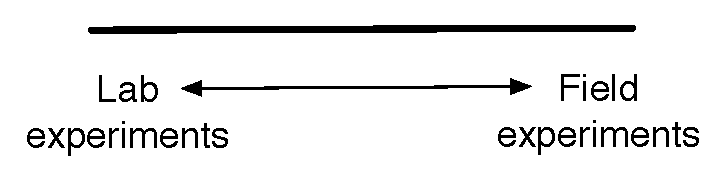
\includegraphics[width=0.7\textwidth]{figures/experiments_design_space_1d.pdf}}
\only<2>{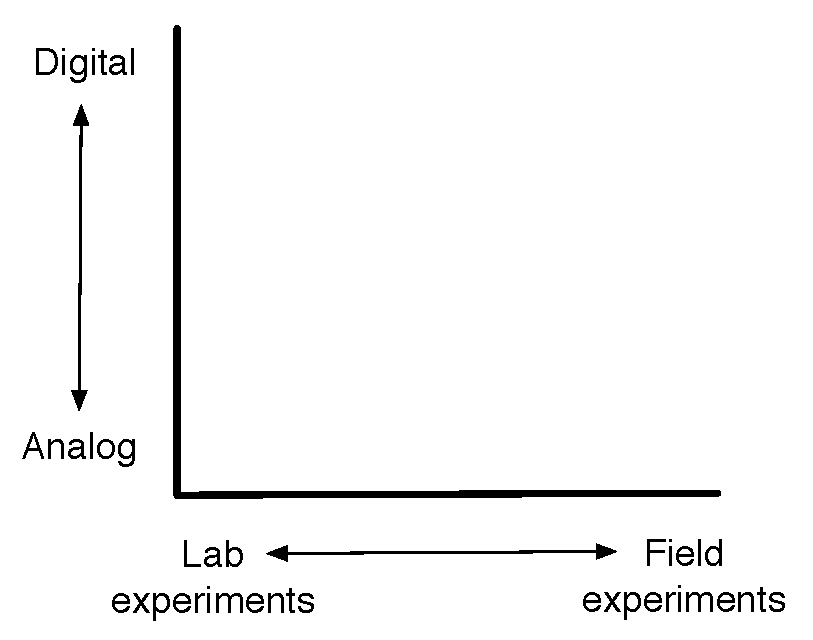
\includegraphics[width=0.7\textwidth]{figures/experiments_design_space_2d.pdf}}
\end{center}

\end{frame}
%%%%%%%%%%%%%%%%%%%%%%%
\begin{frame}

Experiments have four main ingredients:
\begin{itemize}
\item recruiting participants \pause
\item randomization treatment \pause
\item delivering treatment and control \pause
\item measuring outcomes 
\end{itemize}

\end{frame}
%%%%%%%%%%%%%%%%%%%%%%%%
\begin{frame}

Both experiments you read put a lot of care into creating the control group.
\begin{itemize}
\item Voting paper by Nickerson: compared Get-out-the-Vote message to Recycling message \pause
\item Emotional contagion paper by Kramer et al.: a control group for positivity reduced condition and a control group for negatively reduced condition because of different base rates (e.g., 22.4\% of posted had negative words, 46.8\% had positive words)
\end{itemize}

\end{frame}
%%%%%%%%%%%%%%%%%%%%%%
\begin{frame}

A note on terminology:\\
Perturb and observe experiments vs randomized controlled experiments

\end{frame}
%%%%%%%%%%%%%%%%%%%%%%%%%%
\begin{frame}

These experiments move from the individual to the dyad.

\begin{center}

\includegraphics[width=0.2\textwidth]{figures/point}
\end{center}

\pause

\begin{center}
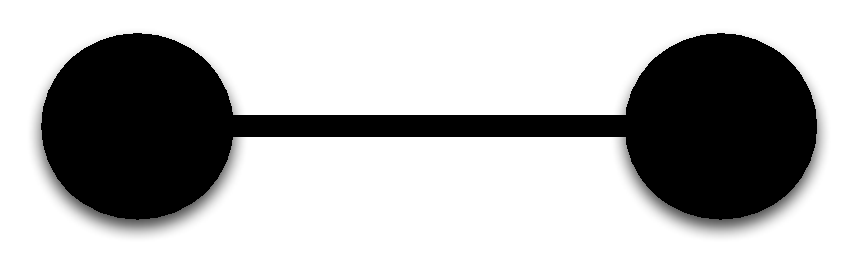
\includegraphics[width=0.5\textwidth]{figures/dyad}
\end{center}

\end{frame}
%%%%%%%%%%%%%%%%%%%%
\begin{frame}

\begin{itemize}
\item ``birds of a feather flock together'' but why? 
\item Experiments are powerful ways to isolate and estimate causal effects
\item \textcolor{blue}{Experiments are powerful but not perfect: internal validity, external validity}
\end{itemize}

\end{frame}
%%%%%%%%%%%%%%%%%%%%%%%%%%%%%%%%%
\begin{frame}

You saw internal validity and external validity were categories to organize concerns. Explicit in Nickerson study on voting; implicit in Kramer et al.\ study of emotions

\end{frame}
%%%%%%%%%%%%%%%%%%%%%%%%%%%%%%%%%
\begin{frame}

\begin{itemize}
\item ``birds of a feather flock together'' but why? 
\item Experiments are powerful ways to isolate and estimate causal effects
\item Experiments are powerful but not perfect: internal validity, external validity
\end{itemize}

\vfill
Given that common background let's dive in

\end{frame}


\end{document}
